\section{Introduction}

The purpose of this paper is to present the current status of the
system presented in \cite{kroger08:rameau}, Rameau. The system was
first designed for automatic harmonic analysis, but it has been
extended with basic support for computational musicology as well.

%de sétimas, e estudo das cadências finais em 366 dos 371 corais de
%Bach na edição de Riemenschneider \cite{bach41:371}. Cinco corais

% objetivo nao é apresentar resultados, melhor dados
% resultados previos em \cite{kroger08:musicologia}

% tied to chorales

\section{The system}
\label{sec:system}

Rameau has two basic interfaces; the command line interface gives the
user access to all options and functionality and the web interface is
just a basic front-end where the user can either choose a file to be
analyzed, or type the notes of a four-part chorale.

Rameau has nine algorithms for chord finding and four algorithms for
roman numeral analysis. Figures \ref{fig:chord-name-analysis} and
\ref{fig:roman-analysis} show the analysis result for the chord
finding and roman numeral analysis of the chorale 130 in the
Riemenschneider edition \cite{bach41:371} , respectively. Each row
shows the result for one algorithm and the last row show the expected
answer, as predicted \nota{usar verbo melhor} in the answer sheet.
Rameau can output the result in a text-only table or in an annotated
score using LilyPond \cite{nienhuys.ea08:LilyPond} to render the
score. It is noteworthy that the decision tree, k-nearest-neighbor,
and the neural net algorithms have a 100\% accuracy in this chorale.

The answer sheet is as simple ASCII file with the chords names or the
roman numerals. The format is familiar to students of harmony classes,
the only major difference is that the numbers to indicate intervals
are separated by a dot (where they are usually pilled on top of each
other in a graphical representation). For instance, a C major chord
with 7th, 9th, and 13th is represented as C7.9.13. The following is
the complete answer sheet for the chord name analysis of chorale
\#130:

\begin{verbatim}
Em D/F# G B7/F# Em B/D# C/E D7/F# [A] Em7
Am7/C Am7 D G G G/B D D Am/C Em/B [A] B 
B7 Em
\end{verbatim}

and the complete answer sheet for the roman numeral analysis is:

\begin{verbatim}
e: i V6/III III V4.3 i V6 VI6 V6.5/III
III i G: ii6.5 ii7 V I I I6 V -
e: iv6 i6.4 - V7 - i
\end{verbatim}

\begin{figure}
  \centering
  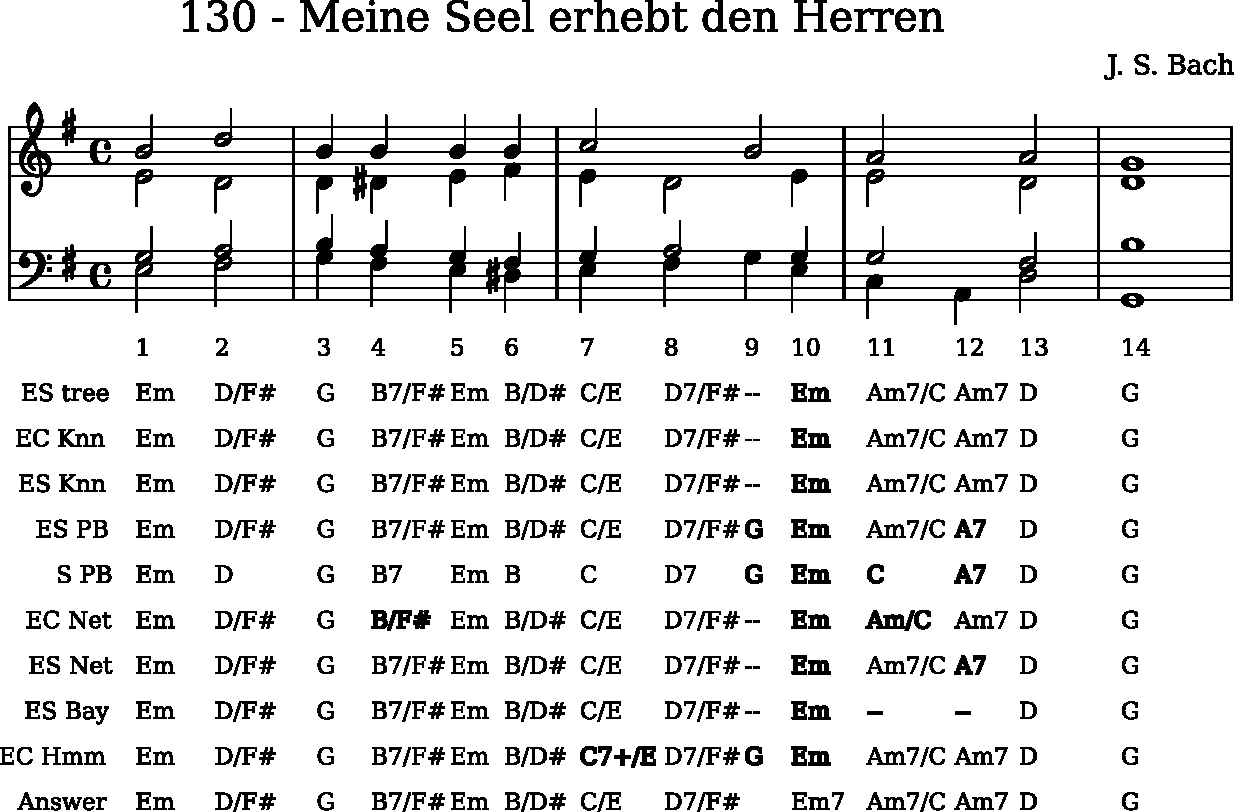
\includegraphics[scale=0.4]{analysis-130}
  \caption{Chord name analysis}
  \label{fig:chord-name-analysis}
\end{figure}
\begin{figure}
  \centering
  \includegraphics[scale=0.4]{analysis-functional-130}  
  \caption{Roman numeral analysis}
  \label{fig:roman-analysis}
\end{figure}

\section{Algorithms}
\label{sec:algorithms}

Rameau includes implementations of some chord labeling and roman
numeral analysis algorithms. Among them are a hidden Markov model
\cite{raphael.ea03:harmonic}, a reimplementation of Pardo \&
Birmingham's algorithm \cite{pardo.ea99:automated}, neural networks
\cite{tsui02:harmonic}, a port of Temperley and Sleator's ``melisma''
root-finding algorithm \cite{temperley.ea99:modeling}, and some other
machine learning techniques.

The machine learning algorithms in Rameau can be tuned by command-line
parameters, and also retrained with different data sets. Also, more
than one version of each algorithm may be compiled in Rameau, and each
such version can be specifically prepared to perform better in some
condition.

\section{Computational musicology}
\label{sec:comp-music}

%% and visualization

We have implemented a few musicological functions in Rameau. The goal
is to turn Rameau into a full framework for computational musicology.

The commands ``octaves'' and ``fifths'' show how many consecutive
octaves and fifths are in a piece and where they are. These functions
can generate lilypond scores of the passage where the octaves or
fifths happens, making it easy to visualize the results. We found, for
instance, that all consecutive octaves in Bach Chorales are in the
form unison--octave or octave--unison (see fig.
\ref{fig:oitavas-e-unissonos}), but no consecutive octaves in all
Chorales are parallel, although a few fifths are (in chorales 4, 46,
71, and 266).

\begin{figure}[!h]
  \centering
  \subfloat[Chorale \#244]{
    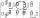
\includegraphics[scale=1]{244-oitava}
    \label{fig:244-oitava}
  }
  \qquad
  \subfloat[Chorale \#279]{
    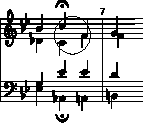
\includegraphics[scale=1]{279-oitava}
    \label{fig:279-oitava}
  }
  \qquad
  \subfloat[Chorale \#329]{
    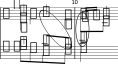
\includegraphics[scale=1]{329-oitava}
    \label{fig:329-oitava}
  }
  \caption{Consecutive octaves and unisons}
  \label{fig:oitavas-e-unissonos}
\end{figure}

The command ``chords'' list the frequency of each type of chord in a
set of chorales. For instance, the type of chords in chorale \#130
can be seen in the following list:

\begin{verbatim}
 C/F#                : 4.2% (1 of 24)
 C/D#                : 4.2% (1 of 24)
 C/E                 : 4.2% (1 of 24)
 Cm7/C               : 4.2% (1 of 24)
 Cm7                 : 4.2% (1 of 24)
 C/B                 : 4.2% (1 of 24)
 Cm/C                : 4.2% (1 of 24)
 Cm/B                : 4.2% (1 of 24)
 C7                  : 4.2% (1 of 24)
 C7/F#               : 8.3% (2 of 24)
 --                  : 8.3% (2 of 24)
 Cm                  : 16.7% (4 of 24)
 C                   : 29.2% (7 of 24)
\end{verbatim}

Not surprisingly, the major and minor triad account for the majority
of chord types. But more than 8.3\% are non-chords (marked with a
double dash), since things listed as chords like C7/F$\sharp$ and
C/D$\sharp$ are probably non-chord tones as well. With this command we
can inspect what are the most used types of sonorities, besides the
major and minor triads.

The command ``crossings'' find passages where are voice crossings. We
found that there are some kind of voice crossing in 57\% of the Bach
Chorales, although most of the crossings happen in a short period of
time (no more than two beats). There are a few interesting cases. For
instance, the alto is the lowest voice for a brief period of time
(fig. \ref{fig:035-cruzamento}) in choral \#35 and there is a crossing
of the soprano and alto and tenor and bass (fig.
\ref{fig:290-66-74-cruzamento}).

There are also commands to find the vocal range used in the
composition, to find melodic jumps in a voice (to analyze vocal
writing), to show how the seventh of chords were resolved, and to
collect stats on how many chord progressions found in the chorales are
strong, weak, superstrong and neutral, according to Schoenberg's
theory of harmony.

\begin{figure}[!h]
  \centering
  \subfloat[Chorale \#35]{
    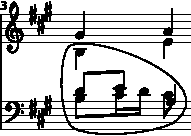
\includegraphics[scale=1]{035-16-20-cruzamento}
    \label{fig:035-cruzamento}
  }
  \subfloat[Chorale \#290]{
    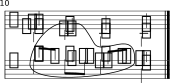
\includegraphics[scale=1]{290-66-74-cruzamento}
    \label{fig:290-66-74-cruzamento}
  }
  \caption{Voice crossing}
  \label{fig:coral-003}
\end{figure}

Finally, rameau can analyze the final cadence of the chorales and list
then. Many commands can generate a cloud representation of its
results. The advantage of such representation is that a lot of data
can be easily ... in just one picture. We can see a cloud
representation for all final cadences in the Bach Chorales in figure
\ref{fig:cadences}. From this figure it is easy to see that the most
common cadence is I ii V I, where ii can be a minor triad or a
half-diminished seventh chord.

\begin{figure}
  \centering
  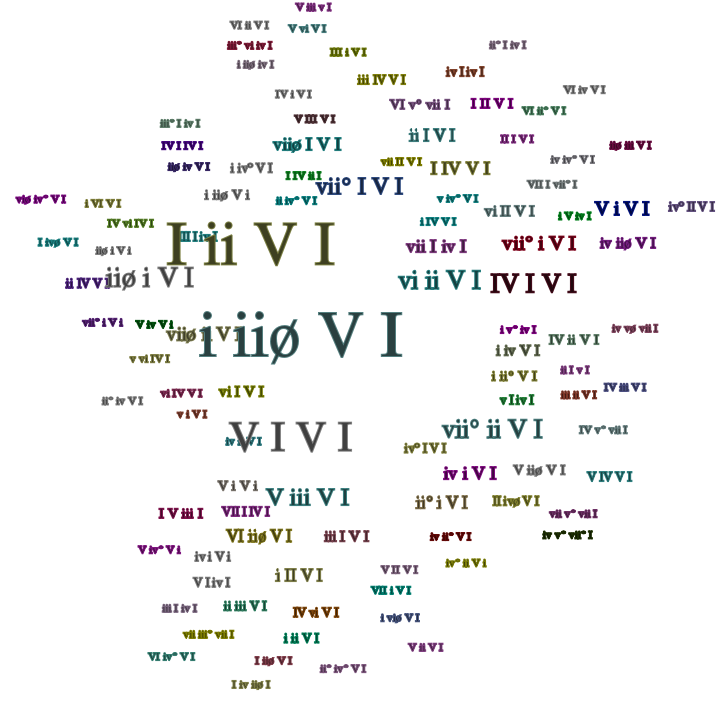
\includegraphics[scale=0.35]{cadences}
  \caption{Final cadences in Bach Chorales}
  \label{fig:cadences}
\end{figure}

\section{Conclusion}
\label{sec:conclusion}

In this paper we presented the current status of rameau, a framework
for automatic harmonic analysis and computational musicology. In this
framework we implemented a few algorithms for chord-finding and roman
numeral analysis and also a few commands for computational musicology.

A system is as good as the input provided to it. Although we published
the preliminary results of using the computational musicology commands
in the 371 Bach Chorales, we found and corrected a large amount of
errors in our input data, so much that we are not confortable in
publishing any more results until we correct the corpus to a level
that makes us more confident. We are in the process of correcting all
371 chorales against the Budapest edition, that some musicologists
find reliable \cite{fitsioris.ea08:parallel}.

Also, the functions for musicology need to be further tested, debuged,
and refined. The rameau architeture is too tied to 4-voice part
writing. We plan to address these problems in a future release of
rameau.

%%% Local Variables: 
%%% mode: latex
%%% TeX-master: "icmc2009"
%%% End: 
